%%
%% Author: s153576
%% 15-12-2017
%%

\documentclass[language=english,number=]{homework}

\usepackage{graphicx}
\usepackage{float}
\usepackage{listings}
\usepackage{color}
\usepackage{fancyvrb}
\usepackage{algorithm}
\usepackage{algpseudocode}
\usepackage{parskip}

\coursename{Introduction to Cryptology}
\author{Sophie van den Eerenbeemt\\0954445}
\date{\today}

% Document
\begin{document}
    \maketitlepage

    Goal of encryption:
    \begin{itemize}
        \item Provide confidentiality.
    \end{itemize}

    \section{Encryption schemes}

    \subsection{Substitution cipher}

    Replace each letter by a symbol or another letter.
    This is a \textit{permutation}.

    \textbf{Algorithm}: permute alphabet

    \textbf{Key}: which permutation you use

    Attacks:
    \begin{itemize}
        \item \textit{Brute force attack}: decrypt with all possible keys until something readable occurs.
        This leads to a total of $26!$ possible keys.
        \item \textit{Frequency analysis} of the occurring symbols.
    \end{itemize}

    Substitution leads to \textit{confusion}.
    It should not be used by itself, because of frequency analyis.

    Gets stronger when the key gets longer relative to message size and when there is more randomness in the key.

    \subsection{Transposition cypher}

    We reorder the message.
    Transposition leads to \textit{diffusion}.

    Confusion and diffusion are the building blocks of encryption.
    When encrypting, we use confusion and diffusion to destroy structure as much as possible.

    \subsection{Column transposition}

    Key permutation of number of colums.
    Add x on remaining blancs, such that all columns have the same length.

    \textbf{Key}: 2354 means the second column first, third column second, etc.

    \subsection{Caesar cipher}

    \textbf{Algorithm}: shift every letter $k$ to the right in the alphabet.

    \textbf{Key}: $k \in \{1, \dots, 25\}$

    \subsection{Vigenere cipher}

    \textbf{Algorithm}: Use $n$ caesar ciphers:
    \begin{itemize}
        \item key $k_1$ for letters $1, n+1, 2n+1, \dots$
        \item key $k_2$ for letters $2, n+2, 2n+2, \dots$
        \item $\dots$
        \item key $k_n$ for letters $n, 2n, 3n, \dots$
    \end{itemize}
    There are $26^n$ possible keys.

    Usually keys are seen as letters: $a=0$, $b=1$, etc.

    \textbf{Example}
    \begin{itemize}
        \item Key: CRYPTO
        \item Message: SECRET
        \item Encryption: UVA...
    \end{itemize}

    Attacks:
    \begin{itemize}
        \item We assume the text is long enough. We break up the ciphertext in pieces of length $n$ and do frequency analysis on each of $n$ positions.
        This only works if you know $n$.
        \begin{itemize}
            \item \textit{Kasishi's trick}: compute autocorrelation.
            In the cyphertext, rotate by $m$ symbols and count the number of equal symbols in original and rotated texts.
            Equal = in the same position.
            Rotation of $m$ with highest count is most likely the key.
            \item Search for repeated patterns.
            Key is probably a divisor of distance between repeated patterns.
        \end{itemize}
    \end{itemize}

    \subsection{Playfair cipher}

    \textbf{Key}: Build key using the keyword, and the alphabet $a$ through $z$.
    Strip the keyword from repeating letters, and use the remaining word and alphabet to fill up a $5 \times 5$ matrix.
    This is your key.

    \textbf{Algorithm}: In your message, add an `x' in between letters that are repetitive, or at the end if the total number of letters is uneven.
    Split into pairs.
    If two letters are in different rows and different columns, we use the letters in the same row, different columns to encrypt a letter.
    If they are in the same row/column, we rotate one to the right/down and use the rule explained before.

    \subsection{Venom cipher, One Time Pad (OTP)}

    \textbf{Key}: exactly as long as plaintext, and is totally random.

    \textbf{Algorithm}: add key and plaintext $\mod m$, where $m$ is the number of symbols in the alphabet.

    Note that OTP with bits only is adding $\mod 2$, which is the logical XOR.

    \begin{theorem}[Shannon]
        OTP gives perfect security.
        Information-theoretic.
    \end{theorem}

    However, OTP is \textit{impractical}.
    Key is as long as plaintext is useless.
    If we have a short key, we can use non-secure chanel to transport the (short) key, and a non-secure channel for message.
    This is not the case for long keys.

    Note that OPT is visionere with an infinitely long key.

    \textit{Plausible deniability}: one can provide 2 plaintexts, 2 keys that lead to the same ciphertext.
    You can make it plausible that something means something, while actually it means something completely different.You can make your ciphertext mean anything you want.

    Remark: never use a key twice!
    \begin{align*}
        m_1 \oplus k &= c_1 \\
        m_2 \oplus k &= c_2 \\
        m_1 \oplus m_2 &= c_1 \oplus c_2
    \end{align*}
    where $\oplus$ is the logical XOR operation.
    Note that this leaks information about the plaintexts!
    Places where $m_1$ and $m_2$ have equal bits, $c_1 \oplus c_2$ will have a zero bit.

    \subsection{Visual cryptography}

    \textbf{Key}: A black/white picture, totally random.

    \textbf{Algorithm}: Where message picture is black, reverse key picture bit.
    Where message picture is white, copy key picture bit.

    \newpage
    \section{Randomness}

    What is randomness?
    See video of Eureka.

    \textit{Golomb's properties of randomness}: we have a sequence of $n$ bits, $s_0, \dots, s_{n-1}$.
    \begin{itemize}
        \item All possible subsequences (neightouring) of length $k$ are equally likely to occur, i.e. $\approx \frac{n}{2^k}$ times.
        $2^k$ subsequencees of length $n$.
        \item Define a \textit{run} as a subsequence of equal bits, surrounded by different bits.
        Now, the number of runs of length $1$ is $\frac{1}{2}$ the number of runs, the number of runs of length $2$ is $\frac{1}{4}$ the number of runs, the number of runs of length $3$ is $\frac{1}{8}$ the number of runs, etc.

        Leads to a total number of runs of $\approx \frac{n}{2}$.

        Moreover, half of the runs should have zeroes, half of the runs should have ones.

        Note that these first two properties are not independent
        \item Define:
        \begin{align*}
            A(k) &= \# \{i | s_i = s_{i + k \mod n} \} \\
            D(k) &= \# \{i | s_i \ne s_{i + k \mod n} \} \\
            AC(k) &= \frac{A(k) - D(k)}{n} \in [-1,1]
        \end{align*}
        with $k = 0, 1, \dots, n-1$.
        Note that $A(k) + D(k) \approx n$.

        Now, it should hold that
        \[
            \forall $k$ : AC(0) = 1 \wedge AC(k) \approx 0.
        \]
    \end{itemize}

    \newpage
    \section{Generating long keys from short keys}

    \subsection{Stream cipher}

    The basic idea: use a short key and expand it into long stream of pseudorandom bits.

    This is \textit{deterministic}, the stream is periodic, because it uses a finite state of bits.

    \textbf{Algorithm}: a sequence of $n$ bits, $s_0, \dots, s_{n-1}$.
    Every clock tick, $s_0$ is output, all bits shift to the left, and $s_{n-1} = f(s_0, \dots, s_n-1)$.
    This is called \textit{feedback, shift, register}.

    Note that this is \textit{periodic}.
    We want the period to be as close to $2^n$ as we can get, then your period is pretty much `infinite'.

    \subsection{Block cipher}

    \textbf{Input}: key of fixed length, and a message block of fixed length.

    \textbf{Output}: ciphertext, usually of same length as input block.

    For a fixed key $k$, this is a permutation of the set of all possible blocks.
    If not, two messages would encrypt to the same output, and you cannot decrypt anymore.
    So, it has to be a permutation.
    The number of blocks is $2^{\text{block length}}$.

    Practical issues:
    \begin{itemize}
        \item Padding: e.g. append a $1$ bit and as many $0$ bits as needed
        \item Divide: up padded message into blocks
        \item Mode of operation: how to deal with multiple blocks
    \end{itemize}

    \subsubsection{Output Feedback Mode}

    Mode of operation, where we start with initial vector $IV_0$, with length is equal to the block length.
    See Figure~\ref{ofm}.
    It gives you a random strea, as long as possible.

    \begin{figure}
        \centering
        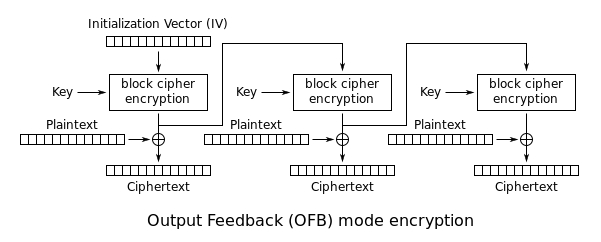
\includegraphics[width=\textwidth]{ofm.PNG}
        \caption{Output Feedback Mode encryption}
        \label{ofm}
    \end{figure}

    \subsubsection{CTR}

    See Figure~\ref{ctr}.
    Here, the nonce is the IV.

    \begin{figure}
        \centering
        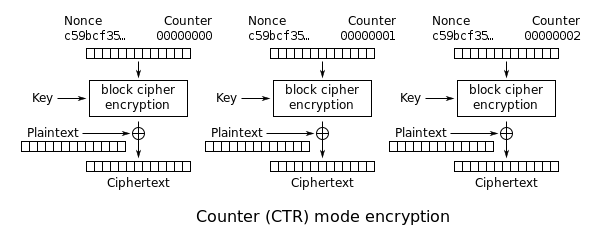
\includegraphics[width=\textwidth]{ctr.PNG}
        \caption{CTR (counter) encryption}
        \label{ctr}
    \end{figure}

    IV requirements:
    \begin{itemize}
        \item not secret
        \item not random
        \item don't reuse! (see OTP)
    \end{itemize}

    \subsection{FSR}

    Stream cipher, designed for hardware.

    \textbf{Algorithm}: we use a register of $n$ bits, $s_0, \dots, s_{n-1}$.
    On one clock tick, $s_0$ is output, all registers shift one to the left, and $s_{n-1} = ff(s_0, \dots, s_{n-1})$, where $ff$ is the \textit{feedback function}.

    \textbf{Example}
    Key is an intitial state, $s_0, s_1, s_2, s_3$.
    Key length is $n$.
    \[
        ff(s_0, s_1, s_2, s_3) = s_0 + s_1 \cdot s_2 + s_3.
    \]
    Example key is $1010$.
    See Table~\ref{exFSR}.

    \begin{table}
        \centering
        \begin{tabular}{c|c|c}
            output & state & ff \\ \hline
            & 1010 &0 \\
            1 & 0100 & 1 \\
            0 & 1001 & 1 \\
            1 & 0011 & 0 \\
            0 & 0110 & 0 \\
            0 & 1100 & 0 \\
            1 & 1000 & 0 \\
            1 & 0000 & 1 \\
            0 & 0001 & 0 \\
            0 & 0010 & 1 \\
            0 & 0101 & 0 \\
            0 & 1010 & \\
        \end{tabular}
        \caption{Example FSR}
        \caption{exFSR}
    \end{table}
    Note that this initial state has a period of 11.
    We have not had all possible states yet.
    5 left, see Table~\ref{exFSR2}.

    \begin{table}
        \centering
        \begin{tabular}{c|c|c}
            output & state & ff \\ \hline
            & 1111 & 0 \\
            1 & 1110 & 1 \\
            1 & 1101 & 1 \\
            1 & 1011 & 1 \\
            1 & 0111 & 1 \\
            0 & 1111 &
        \end{tabular}
        \caption{Example 2 of FSR}
        \caption{exFSR2}
    \end{table}

    \begin{definition}[Periodic]
        Let $(s_i)_{i=0}^{\infty}$ be a sequence.
        $(s_i)$ is periodic if
        \[
            \exists r > 0 : s_{i+r} = s_i \forall i > 0
        \]
        If $r$ is minimal, then $r$ is called the \textit{period}, and $s_0, \dots, s_{r-1}$ is also called the \textit{period}.
    \end{definition}

    \begin{definition}[Ultimately periodic]
        $(s_i)$ is called ultimately periodic if
        \[
            \exists r > 0, i_0 > 0 : s_{i+r} = s_{i} \forall i \ge i_0
        \]
        If both $r, i_0$ minimal, then $s_0, \dots, s_{i_0 - 1}$ is called the \textit{pre-period} and $s_{i_0}, \dots, s_{i_0 + r-1}$ is called \textit{period}.
    \end{definition}

    \begin{theorem}
        Any outputs stream of FSR on $n$ bits is (ultimately) periodic with period $\le 2^n$.
    \end{theorem}
    \begin{proof}
        After $2^{n}+1$ states, there are at least two equal states.
        So, the period is in between those states.
    \end{proof}

    \textbf{Observation} either output stream is periodic or there is at least one state with at least two predecessors.

    \begin{theorem}
        If $(s_i)$ has period $r$ and for some $l > 0$ geldt $s_{i+l} = s_i \forall i \ge i_0$ for some $i_0$ then $r | l$, i.e. $l$ is a multiple of $r$.
    \end{theorem}
    \begin{proof}
        $l = t \cdot r + r_0$, where $0 \le r_0 < r$.
        Forall i big enough:
        \begin{align*}
            s_i &= s_{i+l} \\
            &= s_{i+tr + r_0} \\
            &= s_{i + (t-1)r + r_o} \\
            &= \dots \\
            &= s_{i+r_0}
        \end{align*}

        Then r is minimal, but $r_0$ is smaller, so $r_0 = 0$.
    \end{proof}

    \subsection{LFSR}


\end{document}